%%%%%%%%%%%%%%%%%%%%%%%%%%%%%%%%%%%%%%%%%
% The Legrand Orange Book
% LaTeX Template
% Version 2.4 (26/09/2018)
%
% This template was downloaded from:
% http://www.LaTeXTemplates.com
%
% Original author:
% Mathias Legrand (legrand.mathias@gmail.com) with modifications by:
% Vel (vel@latextemplates.com)
%
% License:
% CC BY-NC-SA 3.0 (http://creativecommons.org/licenses/by-nc-sa/3.0/)
%
% Compiling this template:
% This template uses biber for its bibliography and makeindex for its index.
% When you first open the template, compile it from the command line with the
% commands below to make sure your LaTeX distribution is configured correctly:
%
% 1) pdflatex main
% 2) makeindex main.idx -s StyleInd.ist
% 3) biber main
% 4) pdflatex main x 2
%
% After this, when you wish to update the bibliography/index use the appropriate
% command above and make sure to compile with pdflatex several times
% afterwards to propagate your changes to the document.
%
% This template also uses a number of packages which may need to be
% updated to the newest versions for the template to compile. It is strongly
% recommended you update your LaTeX distribution if you have any
% compilation errors.
%
% Important note:
% Chapter heading images should have a 2:1 width:height ratio,
% e.g. 920px width and 460px height.
%
%%%%%%%%%%%%%%%%%%%%%%%%%%%%%%%%%%%%%%%%%

%----------------------------------------------------------------------------------------
%	PACKAGES AND OTHER DOCUMENT CONFIGURATIONS
%----------------------------------------------------------------------------------------

\documentclass[11pt,fleqn]{book} % Default font size and left-justified equations

%%%%%%%%%%%%%%%%%%%%%%%%%%%%%%%%%%%%%%%%%
% The Legrand Orange Book
% Structural Definitions File
% Version 2.1 (26/09/2018)
%
% Original author:
% Mathias Legrand (legrand.mathias@gmail.com) with modifications by:
% Vel (vel@latextemplates.com)
%
% This file was downloaded from:
% http://www.LaTeXTemplates.com
%
% License:
% CC BY-NC-SA 3.0 (http://creativecommons.org/licenses/by-nc-sa/3.0/)
%
%%%%%%%%%%%%%%%%%%%%%%%%%%%%%%%%%%%%%%%%%

%----------------------------------------------------------------------------------------
%	VARIOUS REQUIRED PACKAGES AND CONFIGURATIONS
%----------------------------------------------------------------------------------------

\usepackage{graphicx} % Required for including pictures
\graphicspath{{Pictures/}} % Specifies the directory where pictures are stored

\usepackage{lipsum} % Inserts dummy text

\usepackage{tikz} % Required for drawing custom shapes
\newcommand*{\ClipSep}{0.3cm}%

\usepackage[portuguese]{babel} % English language/hyphenation

\usepackage{enumitem} % Customize lists
\setlist{nolistsep} % Reduce spacing between bullet points and numbered lists

\usepackage{booktabs} % Required for nicer horizontal rules in tables

\usepackage{xcolor} % Required for specifying colors by name
%\definecolor{ocre}{RGB}{243,102,25} % Define the orange color used for highlighting throughout the book
\definecolor{ocre}{RGB}{49,130,206} % Define the blue color used for highlighting throughout the book

%----------------------------------------------------------------------------------------
%	MARGINS
%----------------------------------------------------------------------------------------

\usepackage{geometry} % Required for adjusting page dimensions and margins

\geometry{
	paper=a4paper, % Paper size, change to letterpaper for US letter size
	top=3cm, % Top margin
	bottom=3cm, % Bottom margin
	left=3cm, % Left margin
	right=3cm, % Right margin
	headheight=14pt, % Header height
	footskip=1.4cm, % Space from the bottom margin to the baseline of the footer
	headsep=10pt, % Space from the top margin to the baseline of the header
	%showframe, % Uncomment to show how the type block is set on the page
}

%----------------------------------------------------------------------------------------
%	FONTS
%----------------------------------------------------------------------------------------

\usepackage{avant} % Use the Avantgarde font for headings
%\usepackage{times} % Use the Times font for headings
\usepackage{mathptmx} % Use the Adobe Times Roman as the default text font together with math symbols from the Sym­bol, Chancery and Com­puter Modern fonts

\usepackage{microtype} % Slightly tweak font spacing for aesthetics
\usepackage[utf8]{inputenc} % Required for including letters with accents
\usepackage[T1]{fontenc} % Use 8-bit encoding that has 256 glyphs

%----------------------------------------------------------------------------------------
%	BIBLIOGRAPHY AND INDEX
%----------------------------------------------------------------------------------------

\usepackage[style=numeric,citestyle=numeric,sorting=nyt,sortcites=true,autopunct=true,babel=hyphen,hyperref=true,abbreviate=false,backref=true,backend=biber]{biblatex}
\addbibresource{bibliography.bib} % BibTeX bibliography file
\defbibheading{bibempty}{}

\usepackage{calc} % For simpler calculation - used for spacing the index letter headings correctly
\usepackage{makeidx} % Required to make an index
\makeindex % Tells LaTeX to create the files required for indexing

%----------------------------------------------------------------------------------------
%	MAIN TABLE OF CONTENTS
%----------------------------------------------------------------------------------------
\setcounter{tocdepth}{1}
\usepackage{titletoc} % Required for manipulating the table of contents

\contentsmargin{0cm} % Removes the default margin

% Part text styling (this is mostly taken care of in the PART HEADINGS section of this file)
\titlecontents{part}
	[0cm] % Left indentation
	{\addvspace{20pt}\bfseries} % Spacing and font options for parts
	{}
	{}
	{}

% Chapter text styling
\titlecontents{chapter}
	[1.25cm] % Left indentation
	{\addvspace{12pt}\large\sffamily\bfseries} % Spacing and font options for chapters
	{\color{ocre!60}\contentslabel[\Large\thecontentslabel]{1.25cm}\color{ocre}} % Formatting of numbered sections of this type
	{\color{ocre}} % Formatting of numberless sections of this type
	{\color{ocre!60}\normalsize\;\titlerule*[.5pc]{.}\;\thecontentspage} % Formatting of the filler to the right of the heading and the page number

% Section text styling
\titlecontents{section}
	[1.25cm] % Left indentation
	{\addvspace{3pt}\sffamily\bfseries} % Spacing and font options for sections
	{\contentslabel[\thecontentslabel]{1.25cm}} % Formatting of numbered sections of this type
	{} % Formatting of numberless sections of this type
	{\hfill\color{black}\thecontentspage} % Formatting of the filler to the right of the heading and the page number

% Subsection text styling
\titlecontents{subsection}
	[1.25cm] % Left indentation
	{\addvspace{1pt}\sffamily\small} % Spacing and font options for subsections
	{\contentslabel[\thecontentslabel]{1.25cm}} % Formatting of numbered sections of this type
	{} % Formatting of numberless sections of this type
	{\ \titlerule*[.5pc]{.}\;\thecontentspage} % Formatting of the filler to the right of the heading and the page number

% Figure text styling
\titlecontents{figure}
	[1.25cm] % Left indentation
	{\addvspace{1pt}\sffamily\small} % Spacing and font options for figures
	{\thecontentslabel\hspace*{1em}} % Formatting of numbered sections of this type
	{} % Formatting of numberless sections of this type
	{\ \titlerule*[.5pc]{.}\;\thecontentspage} % Formatting of the filler to the right of the heading and the page number

% Table text styling
\titlecontents{table}
	[1.25cm] % Left indentation
	{\addvspace{1pt}\sffamily\small} % Spacing and font options for tables
	{\thecontentslabel\hspace*{1em}} % Formatting of numbered sections of this type
	{} % Formatting of numberless sections of this type
	{\ \titlerule*[.5pc]{.}\;\thecontentspage} % Formatting of the filler to the right of the heading and the page number

%----------------------------------------------------------------------------------------
%	MINI TABLE OF CONTENTS IN PART HEADS
%----------------------------------------------------------------------------------------

% Chapter text styling
\titlecontents{lchapter}
	[0em] % Left indentation
	{\addvspace{15pt}\large\sffamily\bfseries} % Spacing and font options for chapters
	{\color{ocre}\contentslabel[\Large\thecontentslabel]{1.25cm}\color{ocre}} % Chapter number
	{}
	{\color{ocre}\normalsize\sffamily\bfseries\;\titlerule*[.5pc]{.}\;\thecontentspage} % Page number

% Section text styling
\titlecontents{lsection}
	[0em] % Left indentation
	{\sffamily\small} % Spacing and font options for sections
	{\contentslabel[\thecontentslabel]{1.25cm}} % Section number
	{}
	{}

% Subsection text styling (note these aren't shown by default, display them by searchings this file for tocdepth and reading the commented text)
\titlecontents{lsubsection}
	[.5em] % Left indentation
	{\sffamily\footnotesize} % Spacing and font options for subsections
	{\contentslabel[\thecontentslabel]{1.25cm}}
	{}
	{}

%----------------------------------------------------------------------------------------
%	HEADERS AND FOOTERS
%----------------------------------------------------------------------------------------

\usepackage{fancyhdr} % Required for header and footer configuration

\pagestyle{fancy} % Enable the custom headers and footers

\renewcommand{\chaptermark}[1]{\markboth{\sffamily\normalsize\bfseries\chaptername\ \thechapter.\ #1}{}} % Styling for the current chapter in the header
\renewcommand{\sectionmark}[1]{\markright{\sffamily\normalsize\thesection\hspace{5pt}#1}{}} % Styling for the current section in the header

\fancyhf{} % Clear default headers and footers
\fancyhead[LE,RO]{\sffamily\normalsize\thepage} % Styling for the page number in the header
\fancyhead[LO]{\rightmark} % Print the nearest section name on the left side of odd pages
\fancyhead[RE]{\leftmark} % Print the current chapter name on the right side of even pages
%\fancyfoot[C]{\thepage} % Uncomment to include a footer

\renewcommand{\headrulewidth}{0.5pt} % Thickness of the rule under the header

\fancypagestyle{plain}{% Style for when a plain pagestyle is specified
	\fancyhead{}\renewcommand{\headrulewidth}{0pt}%
}

% Removes the header from odd empty pages at the end of chapters
\makeatletter
\renewcommand{\cleardoublepage}{
\clearpage\ifodd\c@page\else
\hbox{}
\vspace*{\fill}
\thispagestyle{empty}
\newpage
\fi}

%----------------------------------------------------------------------------------------
%	THEOREM STYLES
%----------------------------------------------------------------------------------------

\usepackage{amsmath,amsfonts,amssymb,amsthm} % For math equations, theorems, symbols, etc

\newcommand{\intoo}[2]{\mathopen{]}#1\,;#2\mathclose{[}}
\newcommand{\ud}{\mathop{\mathrm{{}d}}\mathopen{}}
\newcommand{\intff}[2]{\mathopen{[}#1\,;#2\mathclose{]}}
\renewcommand{\qedsymbol}{$\blacksquare$}
\newtheorem{notation}{Notation}[chapter]

% Boxed/framed environments
\newtheoremstyle{ocrenumbox}% Theorem style name
{0pt}% Space above
{0pt}% Space below
{\normalfont}% Body font
{}% Indent amount
{\small\bf\sffamily\color{ocre}}% Theorem head font
{\;}% Punctuation after theorem head
{0.25em}% Space after theorem head
{\small\sffamily\color{ocre}\thmname{#1}\nobreakspace\thmnumber{\@ifnotempty{#1}{}\@upn{#2}}% Theorem text (e.g. Theorem 2.1)
\thmnote{\nobreakspace\the\thm@notefont\sffamily\bfseries\color{black}---\nobreakspace#3.}} % Optional theorem note

\newtheoremstyle{blacknumex}% Theorem style name
{5pt}% Space above
{5pt}% Space below
{\normalfont}% Body font
{} % Indent amount
{\small\bf\sffamily}% Theorem head font
{\;}% Punctuation after theorem head
{0.25em}% Space after theorem head
{\small\sffamily{\tiny\ensuremath{\blacksquare}}\nobreakspace\thmname{#1}\nobreakspace\thmnumber{\@ifnotempty{#1}{}\@upn{#2}}% Theorem text (e.g. Theorem 2.1)
\thmnote{\nobreakspace\the\thm@notefont\sffamily\bfseries---\nobreakspace#3.}}% Optional theorem note

\newtheoremstyle{blacknumbox} % Theorem style name
{0pt}% Space above
{0pt}% Space below
{\normalfont}% Body font
{}% Indent amount
{\small\bf\sffamily}% Theorem head font
{\;}% Punctuation after theorem head
{0.25em}% Space after theorem head
{\small\sffamily\thmname{#1}\nobreakspace\thmnumber{\@ifnotempty{#1}{}\@upn{#2}}% Theorem text (e.g. Theorem 2.1)
\thmnote{\nobreakspace\the\thm@notefont\sffamily\bfseries---\nobreakspace#3.}}% Optional theorem note

% Non-boxed/non-framed environments
\newtheoremstyle{ocrenum}% Theorem style name
{5pt}% Space above
{5pt}% Space below
{\normalfont}% Body font
{}% Indent amount
{\small\bf\sffamily\color{ocre}}% Theorem head font
{\;}% Punctuation after theorem head
{0.25em}% Space after theorem head
{\small\sffamily\color{ocre}\thmname{#1}\nobreakspace\thmnumber{\@ifnotempty{#1}{}\@upn{#2}}% Theorem text (e.g. Theorem 2.1)
\thmnote{\nobreakspace\the\thm@notefont\sffamily\bfseries\color{black}---\nobreakspace#3.}} % Optional theorem note
\makeatother

% Defines the theorem text style for each type of theorem to one of the three styles above
\newcounter{dummy}
\numberwithin{dummy}{section}
\theoremstyle{ocrenumbox}
\newtheorem{theoremeT}[dummy]{Theorem}
\newtheorem{problem}{Problem}[chapter]
\newtheorem{exerciseT}{Exercise}[chapter]
\theoremstyle{blacknumex}
\newtheorem{exampleT}{Example}[chapter]
\theoremstyle{blacknumbox}
\newtheorem{vocabulary}{Vocabulary}[chapter]
\newtheorem{definitionT}{Definition}[section]
\newtheorem{corollaryT}[dummy]{Corollary}
\theoremstyle{ocrenum}
\newtheorem{proposition}[dummy]{Proposition}

%----------------------------------------------------------------------------------------
%	DEFINITION OF COLORED BOXES
%----------------------------------------------------------------------------------------

% \RequirePackage[framemethod=default]{mdframed} % Required for creating the theorem, definition, exercise and corollary boxes
\RequirePackage[framemethod=tikz]{mdframed} % Required for creating the theorem, definition, exercise and corollary boxes

% Theorem box
\newmdenv[skipabove=7pt,
skipbelow=7pt,
backgroundcolor=black!5,
linecolor=ocre,
innerleftmargin=5pt,
innerrightmargin=5pt,
innertopmargin=5pt,
leftmargin=0cm,
rightmargin=0cm,
innerbottommargin=5pt]{tBox}

% Exercise box
\newmdenv[skipabove=7pt,
skipbelow=7pt,
rightline=false,
leftline=true,
topline=false,
bottomline=false,
backgroundcolor=ocre!10,
linecolor=ocre,
innerleftmargin=5pt,
innerrightmargin=5pt,
innertopmargin=5pt,
innerbottommargin=5pt,
leftmargin=0cm,
rightmargin=0cm,
linewidth=4pt]{eBox}

% Definition box
\newmdenv[skipabove=7pt,
skipbelow=7pt,
rightline=false,
leftline=true,
topline=false,
bottomline=false,
linecolor=ocre,
innerleftmargin=5pt,
innerrightmargin=5pt,
innertopmargin=0pt,
leftmargin=0cm,
rightmargin=0cm,
linewidth=4pt,
innerbottommargin=0pt]{dBox}

% Corollary box
\newmdenv[skipabove=7pt,
skipbelow=7pt,
rightline=false,
leftline=true,
topline=false,
bottomline=false,
linecolor=gray,
backgroundcolor=black!5,
innerleftmargin=5pt,
innerrightmargin=5pt,
innertopmargin=5pt,
leftmargin=0cm,
rightmargin=0cm,
linewidth=4pt,
innerbottommargin=5pt]{cBox}

% Creates an environment for each type of theorem and assigns it a theorem text style from the "Theorem Styles" section above and a colored box from above
\newenvironment{theorem}{\begin{tBox}\begin{theoremeT}}{\end{theoremeT}\end{tBox}}
\newenvironment{exercise}{\begin{eBox}\begin{exerciseT}}{\hfill{\color{ocre}\tiny\ensuremath{\blacksquare}}\end{exerciseT}\end{eBox}}
\newenvironment{definition}{\begin{dBox}\begin{definitionT}}{\end{definitionT}\end{dBox}}
\newenvironment{example}{\begin{exampleT}}{\hfill{\tiny\ensuremath{\blacksquare}}\end{exampleT}}
\newenvironment{corollary}{\begin{cBox}\begin{corollaryT}}{\end{corollaryT}\end{cBox}}

%----------------------------------------------------------------------------------------
%	REMARK ENVIRONMENT
%----------------------------------------------------------------------------------------

\newenvironment{remark}{\par\vspace{10pt}\small % Vertical white space above the remark and smaller font size
\begin{list}{}{
\leftmargin=35pt % Indentation on the left
\rightmargin=25pt}\item\ignorespaces % Indentation on the right
\makebox[-2.5pt]{\begin{tikzpicture}[overlay]
\node[draw=ocre!60,line width=1pt,circle,fill=ocre!25,font=\sffamily\bfseries,inner sep=2pt,outer sep=0pt] at (-15pt,0pt){\textcolor{ocre}{R}};\end{tikzpicture}} % Orange R in a circle
\advance\baselineskip -1pt}{\end{list}\vskip5pt} % Tighter line spacing and white space after remark

%----------------------------------------------------------------------------------------
%	SECTION NUMBERING IN THE MARGIN
%----------------------------------------------------------------------------------------

\makeatletter
\renewcommand{\@seccntformat}[1]{\llap{\textcolor{ocre}{\csname the#1\endcsname}\hspace{1em}}}
\renewcommand{\section}{\@startsection{section}{1}{\z@}
{-4ex \@plus -1ex \@minus -.4ex}
{1ex \@plus.2ex }
{\normalfont\large\sffamily\bfseries}}
\renewcommand{\subsection}{\@startsection {subsection}{2}{\z@}
{-3ex \@plus -0.1ex \@minus -.4ex}
{0.5ex \@plus.2ex }
{\normalfont\sffamily\bfseries}}
\renewcommand{\subsubsection}{\@startsection {subsubsection}{3}{\z@}
{-2ex \@plus -0.1ex \@minus -.2ex}
{.2ex \@plus.2ex }
{\normalfont\small\sffamily\bfseries}}
\renewcommand\paragraph{\@startsection{paragraph}{4}{\z@}
{-2ex \@plus-.2ex \@minus .2ex}
{.1ex}
{\normalfont\small\sffamily\bfseries}}

%----------------------------------------------------------------------------------------
%	PART HEADINGS
%----------------------------------------------------------------------------------------

% Numbered part in the table of contents
\newcommand{\@mypartnumtocformat}[2]{%
	\setlength\fboxsep{0pt}%
	\noindent\colorbox{ocre!20}{\strut\parbox[c][.7cm]{\ecart}{\color{ocre!70}\Large\sffamily\bfseries\centering#1}}\hskip\esp\colorbox{ocre!40}{\strut\parbox[c][.7cm]{\linewidth-\ecart-\esp}{\Large\sffamily\centering#2}}%
}

% Unnumbered part in the table of contents
\newcommand{\@myparttocformat}[1]{%
	\setlength\fboxsep{0pt}%
	\noindent\colorbox{ocre!40}{\strut\parbox[c][.7cm]{\linewidth}{\Large\sffamily\centering#1}}%
}

\newlength\esp
\setlength\esp{4pt}
\newlength\ecart
\setlength\ecart{1.2cm-\esp}
\newcommand{\thepartimage}{}%
\newcommand{\partimage}[1]{\renewcommand{\thepartimage}{#1}}%
\def\@part[#1]#2{%
\ifnum \c@secnumdepth >-2\relax%
\refstepcounter{part}%
\addcontentsline{toc}{part}{\texorpdfstring{\protect\@mypartnumtocformat{\thepart}{#1}}{\partname~\thepart\ ---\ #1}}
\else%
\addcontentsline{toc}{part}{\texorpdfstring{\protect\@myparttocformat{#1}}{#1}}%
\fi%
\startcontents%
\markboth{}{}%
{\thispagestyle{empty}%
\begin{tikzpicture}[remember picture,overlay]%
\node at (current page.north west){\begin{tikzpicture}[remember picture,overlay]%
\fill[ocre!20](0cm,0cm) rectangle (\paperwidth,-\paperheight);
\node[anchor=north] at (4cm,-3.25cm){\color{ocre!40}\fontsize{220}{100}\sffamily\bfseries\thepart};
\node[anchor=south east] at (\paperwidth-1cm,-\paperheight+1cm){\parbox[t][][t]{8.5cm}{
\printcontents{l}{0}{\setcounter{tocdepth}{1}}% The depth to which the Part mini table of contents displays headings; 0 for chapters only, 1 for chapters and sections and 2 for chapters, sections and subsections
}};
\node[anchor=north east] at (\paperwidth-1.5cm,-3.25cm){\parbox[t][][t]{15cm}{\strut\raggedleft\color{white}\fontsize{30}{30}\sffamily\bfseries#2}};
\end{tikzpicture}};
\end{tikzpicture}}%
\@endpart}
\def\@spart#1{%
\startcontents%
\phantomsection
{\thispagestyle{empty}%
\begin{tikzpicture}[remember picture,overlay]%
\node at (current page.north west){\begin{tikzpicture}[remember picture,overlay]%
\fill[ocre!20](0cm,0cm) rectangle (\paperwidth,-\paperheight);
\node[anchor=north east] at (\paperwidth-1.5cm,-3.25cm){\parbox[t][][t]{15cm}{\strut\raggedleft\color{white}\fontsize{30}{30}\sffamily\bfseries#1}};
\end{tikzpicture}};
\end{tikzpicture}}
\addcontentsline{toc}{part}{\texorpdfstring{%
\setlength\fboxsep{0pt}%
\noindent\protect\colorbox{ocre!40}{\strut\protect\parbox[c][.7cm]{\linewidth}{\Large\sffamily\protect\centering #1\quad\mbox{}}}}{#1}}%
\@endpart}
\def\@endpart{\vfil\newpage
\if@twoside
\if@openright
\null
\thispagestyle{empty}%
\newpage
\fi
\fi
\if@tempswa
\twocolumn
\fi}

%----------------------------------------------------------------------------------------
%	CHAPTER HEADINGS
%----------------------------------------------------------------------------------------

% A switch to conditionally include a picture, implemented by Christian Hupfer
\newif\ifusechapterimage
\usechapterimagetrue
\newcommand{\thechapterimage}{}%
\newcommand{\chapterimage}[1]{\ifusechapterimage\renewcommand{\thechapterimage}{#1}\fi}%
\newcommand{\autodot}{.}
\def\@makechapterhead#1{%
{\parindent \z@ \raggedright \normalfont
\ifnum \c@secnumdepth >\m@ne
\if@mainmatter
\begin{tikzpicture}[remember picture,overlay]
\node at (current page.north west)
{\begin{tikzpicture}[remember picture,overlay]
\node[anchor=north west,inner sep=0pt] at (0,0) {\ifusechapterimage\includegraphics[width=\paperwidth]{\thechapterimage}\fi};
\draw[anchor=west] (\Gm@lmargin,-4cm) node [line width=2pt,rounded corners=9pt,draw=ocre,fill=white,fill opacity=0.5,inner sep=15pt]{\strut\makebox[22cm]{}};
\draw[anchor=west] (\Gm@lmargin+.3cm,-4cm) node {\huge\sffamily\bfseries\color{black}\thechapter\autodot~#1\strut};
\end{tikzpicture}};
\end{tikzpicture}
\else
\begin{tikzpicture}[remember picture,overlay]
\node at (current page.north west)
{\begin{tikzpicture}[remember picture,overlay]
\node[anchor=north west,inner sep=0pt] at (0,0) {\ifusechapterimage\includegraphics[width=\paperwidth]{\thechapterimage}\fi};
\draw[anchor=west] (\Gm@lmargin,-9cm) node [line width=2pt,rounded corners=15pt,draw=ocre,fill=white,fill opacity=0.5,inner sep=15pt]{\strut\makebox[22cm]{}};
\draw[anchor=west] (\Gm@lmargin+.3cm,-9cm) node {\huge\sffamily\bfseries\color{black}#1\strut};
\end{tikzpicture}};
\end{tikzpicture}
\fi\fi\par\vspace*{60\p@}}}

%-------------------------------------------

\def\@makeschapterhead#1{%
\begin{tikzpicture}[remember picture,overlay]
\node at (current page.north west)
{\begin{tikzpicture}[remember picture,overlay]
\node[anchor=north west,inner sep=0pt] at (0,0) {\ifusechapterimage\includegraphics[width=\paperwidth]{\thechapterimage}\fi};
\draw[anchor=west] (\Gm@lmargin,-9cm) node [line width=2pt,rounded corners=15pt,draw=ocre,fill=white,fill opacity=0.5,inner sep=15pt]{\strut\makebox[22cm]{}};
\draw[anchor=west] (\Gm@lmargin+.3cm,-9cm) node {\huge\sffamily\bfseries\color{black}#1\strut};
\end{tikzpicture}};
\end{tikzpicture}
\par\vspace*{270\p@}}
\makeatother

%----------------------------------------------------------------------------------------
%	LINKS
%----------------------------------------------------------------------------------------

\usepackage{hyperref}
\hypersetup{hidelinks,backref=true,pagebackref=true,hyperindex=true,colorlinks=false,breaklinks=true,urlcolor=ocre,bookmarks=true,bookmarksopen=false}

\usepackage{bookmark}
\bookmarksetup{
open,
numbered,
addtohook={%
\ifnum\bookmarkget{level}=0 % chapter
\bookmarksetup{bold}%
\fi
\ifnum\bookmarkget{level}=-1 % part
\bookmarksetup{color=ocre,bold}%
\fi
}
}

\usepackage{pdfpages}

\usepackage{float}
\let\origfigure\figure
\let\endorigfigure\endfigure
\renewenvironment{figure}[1][2] {
    \expandafter\origfigure\expandafter[H]
} {
    \endorigfigure
}
\usepackage{caption}
\renewcommand{\figurename}{Figura}

\usepackage{chngpage}
\usepackage{calc}
% \usepackage{mwe}
\usepackage[skins]{tcolorbox}

\renewcommand{\contentsname}{Conteúdo}
\definecolor{dialogoBorder}{RGB}{225, 228, 232}

% Habilitar para ter o comando \roundpic
% Ref: <https://subscription.packtpub.com/book/hardware_and_creative/9781784395148/4/ch04lvl1sec46/shaping-an-image-like-a-circle>
% \newcommand{\roundpic}[4][]{
%   \tikz\node [circle, minimum width = #2,
%     path picture = {
%       \node [#1] at (path picture bounding box.center) {
%         \includegraphics[scale=#3]{#4}};
%     }] {};}
 % Insert the commands.tex file which contains the majority of the structure behind the template

%\hypersetup{pdftitle={Title},pdfauthor={Author}} % Uncomment and fill out to include PDF metadata for the author and title of the book

%----------------------------------------------------------------------------------------

\begin{document}

%----------------------------------------------------------------------------------------
%	TITLE PAGE
%----------------------------------------------------------------------------------------

\begingroup
\thispagestyle{empty} % Suppress headers and footers on the title page
\begin{tikzpicture}[remember picture,overlay]
\node[inner sep=0pt] (background) at (current page.center) {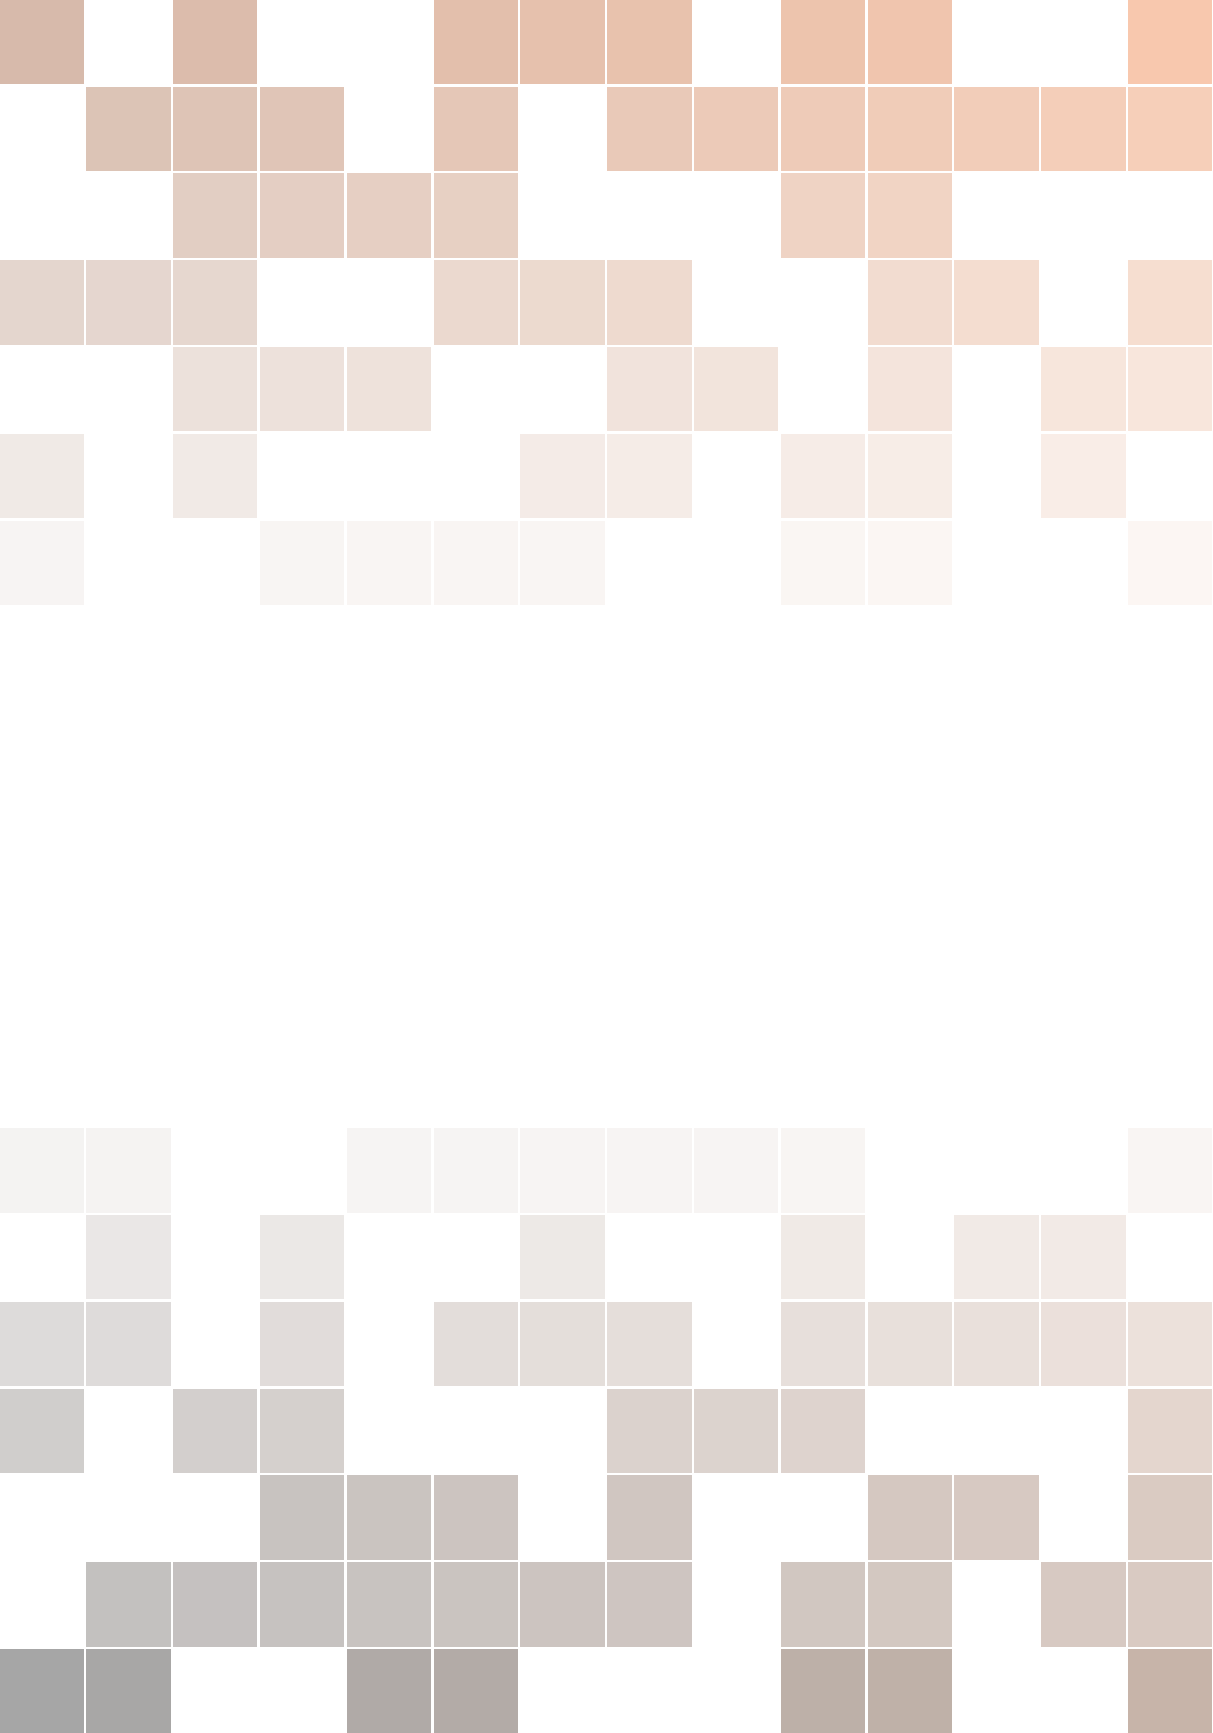
\includegraphics[width=\paperwidth]{background.pdf}};
\draw (current page.center) node [fill=ocre!30!white,fill opacity=0.6,text opacity=1,inner sep=1cm]{\Huge\centering\bfseries\sffamily\parbox[c][][t]{\paperwidth}{\centering Aquele com o glossário de Friends\\[15pt] % Book title
{\Large Entenda as referências da série}\\[20pt] % Subtitle
{\Large Átila \& Sinara}\\[10pt] % Author name
{\Huge CAMURÇA}
}};
\end{tikzpicture}
\vfill
\endgroup

%----------------------------------------------------------------------------------------
%	COPYRIGHT PAGE
%----------------------------------------------------------------------------------------

\newpage
~\vfill
\thispagestyle{empty}

\noindent Copyright \copyright\ 2019 John Smith\\ % Copyright notice

\noindent \textsc{Published by Publisher}\\ % Publisher

\noindent \textsc{https://glossario-friends.netlify.app/}\\ % URL

\noindent Licensed under the Creative Commons Attribution-NonCommercial 3.0 Unported License (the ``License''). You may not use this file except in compliance with the License. You may obtain a copy of the License at \url{http://creativecommons.org/licenses/by-nc/3.0}. Unless required by applicable law or agreed to in writing, software distributed under the License is distributed on an \textsc{``as is'' basis, without warranties or conditions of any kind}, either express or implied. See the License for the specific language governing permissions and limitations under the License.\\ % License information, replace this with your own license (if any)

\noindent \textit{First printing, March 2019} % Printing/edition date

%----------------------------------------------------------------------------------------
%	TABLE OF CONTENTS
%----------------------------------------------------------------------------------------

\usechapterimagefalse % If you don't want to include a chapter image, use this to toggle images off - it can be enabled later with \usechapterimagetrue

\chapterimage{chapter_head_1.pdf} % Table of contents heading image

\pagestyle{empty} % Disable headers and footers for the following pages

\tableofcontents % Print the table of contents itself

\cleardoublepage % Forces the first chapter to start on an odd page so it's on the right side of the book

\pagestyle{fancy} % Enable headers and footers again

%----------------------------------------------------------------------------------------
%	PART
%----------------------------------------------------------------------------------------

\part{Temporada Um}

%----------------------------------------------------------------------------------------
%	CHAPTER 1
%----------------------------------------------------------------------------------------

%\chapterimage{chapter_head_2.pdf} % Chapter heading image

\chapter{Aquele onde Tudo começou}

\graphicspath{{S01/}}
\hypertarget{mr.-potato-head}{%
\section{Mr.~Potato Head}\label{mr.-potato-head}}

\begin{figure}[!ht]
  \begin{adjustwidth}{-\oddsidemargin-1in}{-\rightmargin}
    \centering
    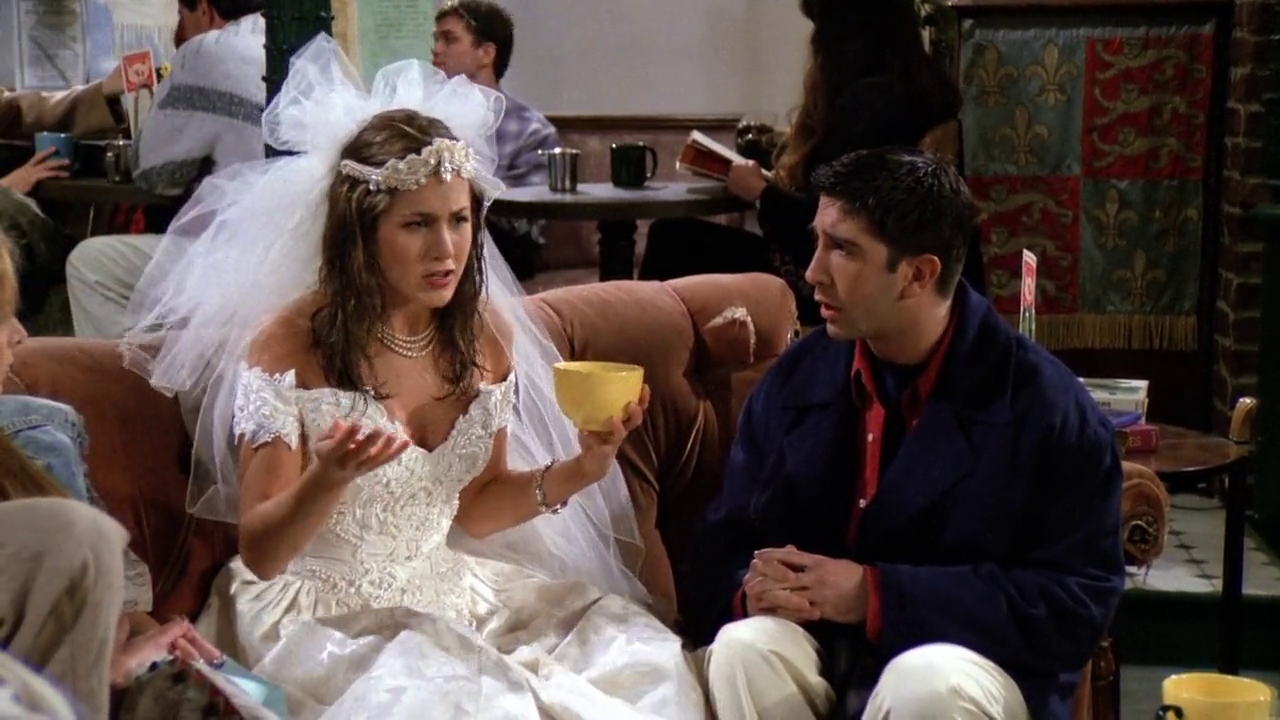
\includegraphics[trim={0 5cm 0 2cm,}, clip, width=\paperwidth]{./S01/img/1/mr-potato-head.png}
    \caption{Mr. Potato Head\label{fig:mr-potato-head}}
  \end{adjustwidth}
\end{figure}

\begin{tcolorbox}[enhanced,center upper,
    drop fuzzy shadow southeast, boxrule=0.3pt,
    lower separated=false,
    colframe=black!30!dialogoBorder,colback=white]
\begin{minipage}[c]{0.14\linewidth}
  \raisebox{\dimexpr-\height+\ht\strutbox\relax}{
    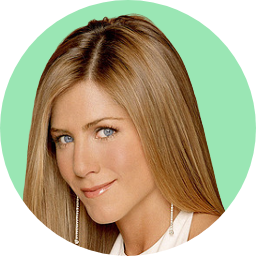
\includegraphics[width=1.5cm]{./assets/img/rachel.png}
  }
   & \centering \scriptsize{Rachel}
\end{minipage}
\hspace{.1mm}
\begin{minipage}[c]{0.8\linewidth}
  \textbf{- [...] and that's when it hit me: How much Barry looks like Mr. Potato Head.}\\
  - [...] e me dei conta: O quanto Barry se parece com o Mr. Potato Head.
\end{minipage}
\end{tcolorbox}

\saveparinfos
\noindent
\begin{minipage}[c]{0.5\textwidth}\useparinfo

Rachel menciona que Barry, seu ex-noivo, parece com o \emph{Mr.~Potato
Head.} Trata-se de um brinquedo inventado por George Lerner, lançado
pela Hasbro em 1952. Em sua versão original havia apenas as partes, tais
como: os olhos, as orelhas e a boca, e era obrigação dos pais fornecerem
uma batata de verdade para formar a cabeça.

O \emph{Mr.~Potato Head} também pode ser visto nos filmes de \emph{Toy
Story} (1995, 1999, 2010, 2019), como um dos brinquedos do Andy.

\end{minipage}\hfill
\begin{minipage}[c]{0.45\textwidth}

\begin{figure}
  \centering
  \begin{tikzpicture}
    \node [inner sep=0pt] at (0,0) {
      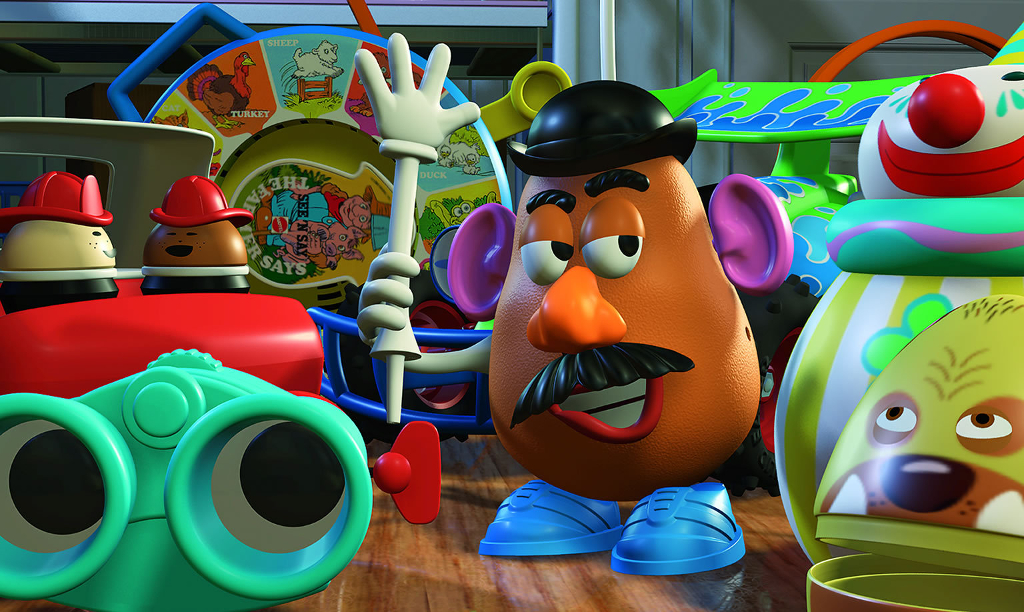
\includegraphics[width=0.8\textwidth,keepaspectratio]{./S01/img/1/mr-potato-head-toy-story.jpg}
    };
    \draw [white, rounded corners=\ClipSep, line width=\ClipSep]
    (current bounding box.north west) --
    (current bounding box.north east) --
    (current bounding box.south east) --
    (current bounding box.south west) -- cycle
    ;
    \end{tikzpicture}
    \caption{Mr. Potato Head (Toy Story)\label{fig:mr-potato-head-toy-story}}
\end{figure}

\end{minipage}

\hypertarget{referuxeancias}{%
\subsection{Referências}\label{referuxeancias}}

\begin{itemize}
\tightlist
\item
  \sloppy V&A Museum of Childhood. \url{https://www.vam.ac.uk/moc/collections/mr-potato-head/}
\item
  \sloppy Toy Story (IMDB). \url{https://www.imdb.com/title/tt0114709/}
\end{itemize}

\hypertarget{tres-destinos}{%
\section{Tres Destinos}\label{tres-destinos}}

\begin{figure}[!ht]
  \begin{adjustwidth}{-\oddsidemargin-1in}{-\rightmargin}
    \centering
    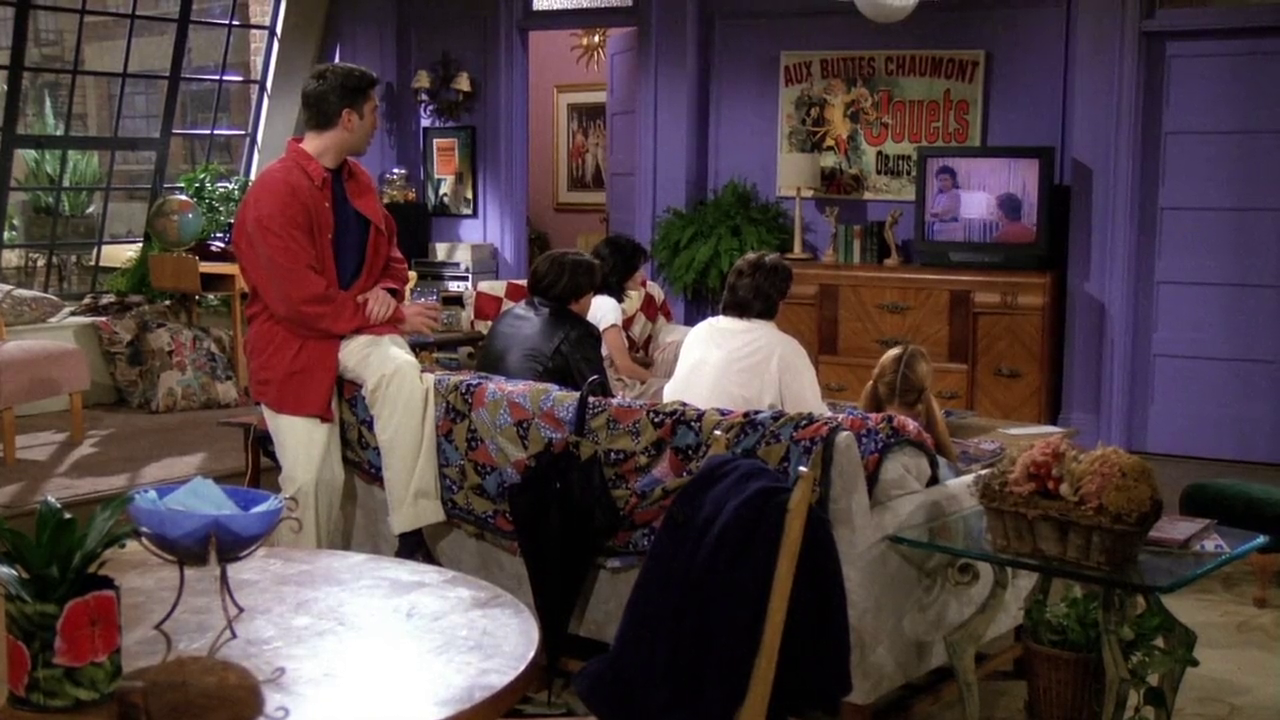
\includegraphics[trim={0 7cm 0 1.5cm,}, clip, width=\paperwidth]{./S01/img/1/tres-destinos.png}
    \caption{Tres Destinos\label{fig:tres-destinos}}
  \end{adjustwidth}
\end{figure}

Os amigos são vistos assistindo a telenovela \emph{Tres Destinos}
(1993), produzida para o mercado hispânico nos Estados Unidos. É a
clássica novela mexicana, do tipo popularmente exibida no Brasil, que
conta a história de 3 jovens irmãs unidas e separadas pelo mesmo homem,
com todos os ingredientes usuais: intriga, paixão, vingança, ódio,
ternura e amor.

\hypertarget{referuxeancias-1}{%
\subsection{Referências}\label{referuxeancias-1}}

\begin{itemize}
\tightlist
\item
  \sloppy EcuRed. \url{https://www.ecured.cu/Tres_destinos_(Telenovela)}
\item
  \sloppy IMDB. \url{https://www.imdb.com/title/tt0211876/}
\item
  \sloppy Abertura (YouTube). \url{https://www.youtube.com/watch?v=kfIk131FZxU}
\end{itemize}

\hypertarget{my-favorite-things}{%
\section{My Favorite Things}\label{my-favorite-things}}

\begin{figure}[!ht]
  \begin{adjustwidth}{-\oddsidemargin-1in}{-\rightmargin}
    \centering
    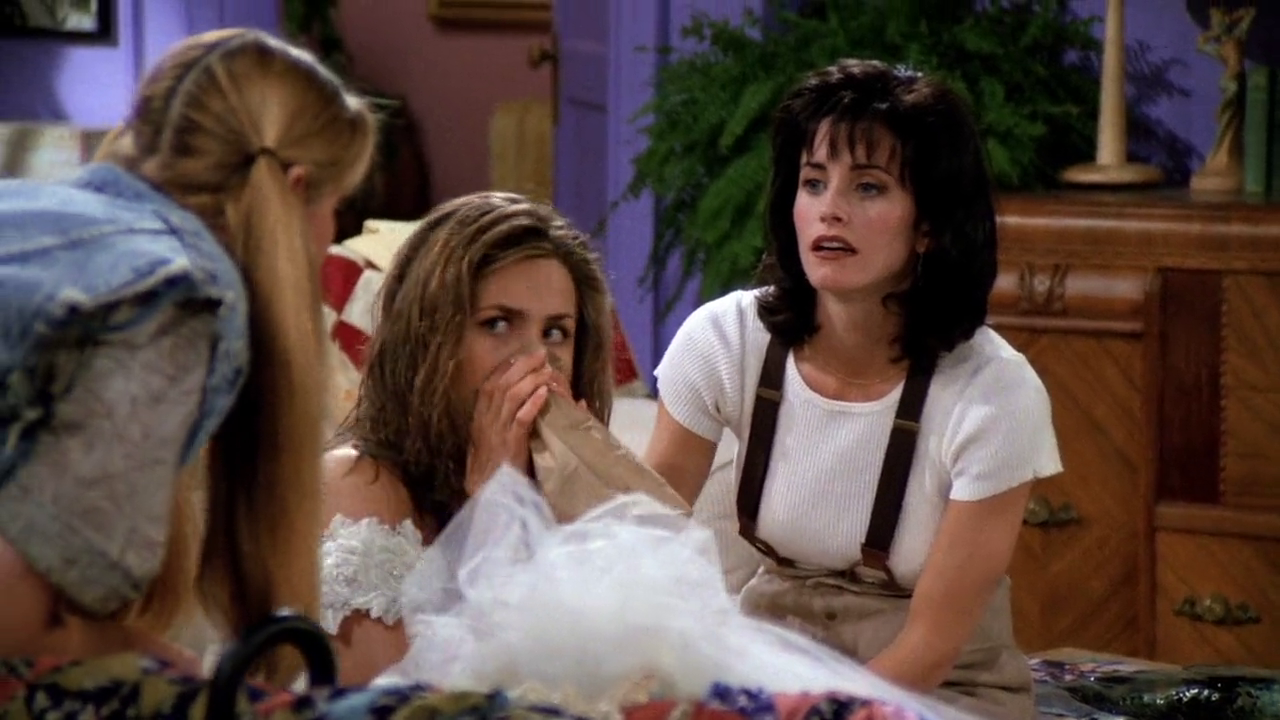
\includegraphics[trim={0 6cm 0 0.5cm,}, clip, width=\paperwidth]{./S01/img/1/my-favorite-things.png}
    \caption{My Favorite Things\label{fig:my-favorite-things}}
  \end{adjustwidth}
\end{figure}

Para acalmar Rachel, Phoebe canta uma versão própria da música \emph{My
Favorite Things} do musical \emph{The Sound of Music} (1959). Em 1965
foi lançado o filme, conhecido no Brasil como \emph{A Noviça Rebelde.}

A música expressa que você deve lembrar de suas coisas favoritas sempre
que se sentir triste.

\bigskip
\begin{tcolorbox}[enhanced,
    drop fuzzy shadow southeast, boxrule=0.3pt,
    lower separated=false, sidebyside, sidebyside align=top,
    halign=flush right, halign lower=left,
    colframe=black!30!dialogoBorder,colback=musicaBg]
\includegraphics[width=0.4cm]{./assets/img/icon-music.png}\\
When I’m feeling sad\\I simply remember my favorite things\\
\tcblower
\includegraphics[width=0.4cm]{./assets/img/icon-language.png}\\
Quando me sinto triste\\Simplesmente lembro de minhas coisas favoritas\\
\end{tcolorbox}

\begin{center}\rule{0.5\linewidth}{0.5pt}\end{center}

Versão da Phoebe:

\bigskip
\begin{tcolorbox}[enhanced,
    drop fuzzy shadow southeast, boxrule=0.3pt,
    lower separated=false, sidebyside, sidebyside align=top,
    halign=flush right, halign lower=left,
    colframe=black!30!dialogoBorder,colback=musicaBg]
\includegraphics[width=0.4cm]{./assets/img/icon-music.png}\\
Raindrops on roses\\And whiskers on kittens\\Doorbells and sleigh bells\\And something with mittens\\La la la la something with strings\\
\tcblower
\includegraphics[width=0.4cm]{./assets/img/icon-language.png}\\
Pingos de chuva em rosas\\E bigodes de gatinhos\\Campainhas e sinos\\E algo com luvas de lã\\La la la la algo com cordas\\
\end{tcolorbox}

Versão original:

\bigskip
\begin{tcolorbox}[enhanced,
    drop fuzzy shadow southeast, boxrule=0.3pt,
    lower separated=false, sidebyside, sidebyside align=top,
    halign=flush right, halign lower=left,
    colframe=black!30!dialogoBorder,colback=musicaBg]
\includegraphics[width=0.4cm]{./assets/img/icon-music.png}\\
Raindrops on roses\\And whiskers on kittens\\Bright copper kettles\\And warm woolen mittens\\Brown paper packages\\Tied up with strings\\
\tcblower
\includegraphics[width=0.4cm]{./assets/img/icon-language.png}\\
Pingos de chuva em rosas\\E bigodes de gatinhos\\Brilhantes tachos de cobre\\E quentes luvas de lã\\Pacotes de papel pardo\\Amarrado com cordas\\
\end{tcolorbox}

\begin{tcolorbox}[enhanced,center upper,
    drop fuzzy shadow southeast, boxrule=0.3pt,
    lower separated=false,
    colframe=black!30!dialogoBorder,colback=white]
\begin{minipage}[c]{0.14\linewidth}
  \raisebox{\dimexpr-\height+\ht\strutbox\relax}{
    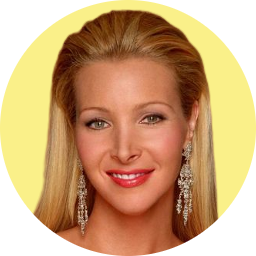
\includegraphics[width=1.5cm]{./assets/img/phoebe.png}
  }
   & \centering \scriptsize{Phoebe}
\end{minipage}
\hspace{.1mm}
\begin{minipage}[c]{0.8\linewidth}
  \textbf{- I helped.}\\
  - Eu ajudei.
\end{minipage}
\end{tcolorbox}

\hypertarget{referuxeancias-2}{%
\subsection{Referências}\label{referuxeancias-2}}

\begin{itemize}
\tightlist
\item
  \sloppy Trecho do filme The Sound of Music, em que é possível ouvir My Favorite Things (Youtube). \url{https://www.youtube.com/watch?v=DGABqdbtQnA}
\item
  \sloppy Wikipédia. \url{https://en.wikipedia.org/wiki/My_Favorite_Things_(song)}
\item
  \sloppy A Noviça Rebelde (IMDB). \url{https://www.imdb.com/title/tt0059742/}
\item
  \sloppy Letra e tradução - Vagalume. \url{https://www.vagalume.com.br/julie-andrews/my-favorite-things-traducao.html}
\end{itemize}

\hypertarget{maina-la-voyante}{%
\section{Maina La Voyante}\label{maina-la-voyante}}

\begin{figure}[!ht]
  \begin{adjustwidth}{-\oddsidemargin-1in}{-\rightmargin}
    \centering
    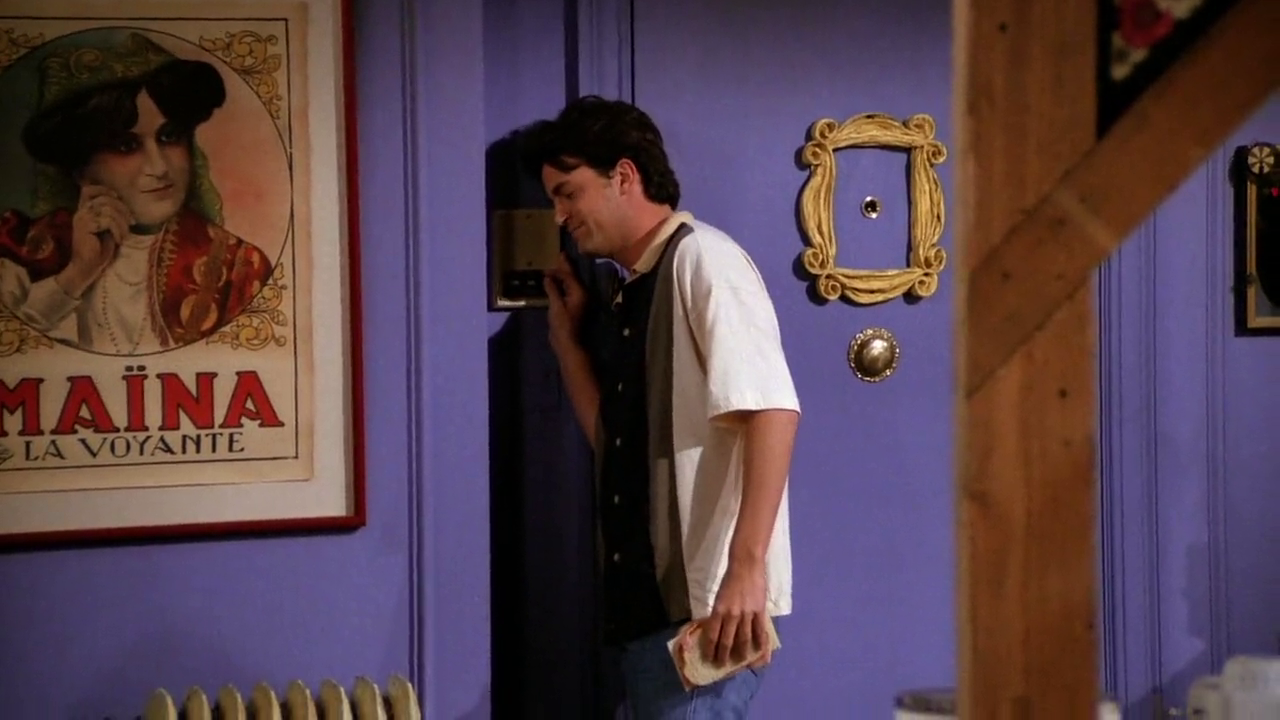
\includegraphics[trim={0 8cm 0 0.5cm,}, clip, width=\paperwidth]{./S01/img/1/maina-la-voyante.png}
    \caption{Maina La Voyante\label{fig:maina-la-voyante}}
  \end{adjustwidth}
\end{figure}

\saveparinfos
\noindent
\begin{minipage}[c]{0.5\textwidth}\useparinfo

Quando Chandler vai atender ao interfone, o poster \emph{Maina La
Voyante} pode ser visto, obra do ilustrador francês Louis Galice
(1864-1935).

\end{minipage}\hfill
\begin{minipage}[c]{0.6\textwidth}

\begin{figure}
  \centering
  \begin{tikzpicture}
    \node [inner sep=0pt] at (0,0) {
      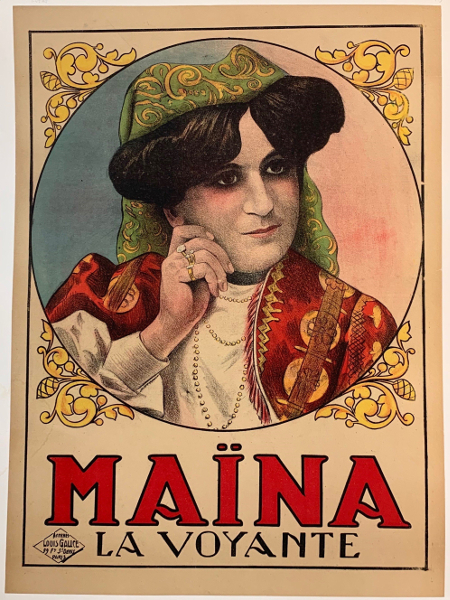
\includegraphics[width=0.6\textwidth,keepaspectratio]{./S01/img/1/maina-la-voyante-poster.jpg}
    };
    \draw [white, rounded corners=\ClipSep, line width=\ClipSep]
    (current bounding box.north west) --
    (current bounding box.north east) --
    (current bounding box.south east) --
    (current bounding box.south west) -- cycle
    ;
    \end{tikzpicture}
    \caption{Maina La Voyante - Poster\label{fig:maina-la-voyante-poster}}
\end{figure}

\end{minipage}

\hypertarget{referuxeancias-3}{%
\subsection{Referências}\label{referuxeancias-3}}

\begin{itemize}
\tightlist
\item
  \sloppy PosterMuseum. \url{https://postermuseum.com/products/maina-la-voyante}
\end{itemize}

\hypertarget{speed-racer}{%
\section{Speed Racer}\label{speed-racer}}

\begin{figure}[!ht]
  \begin{adjustwidth}{-\oddsidemargin-1in}{-\rightmargin}
    \centering
    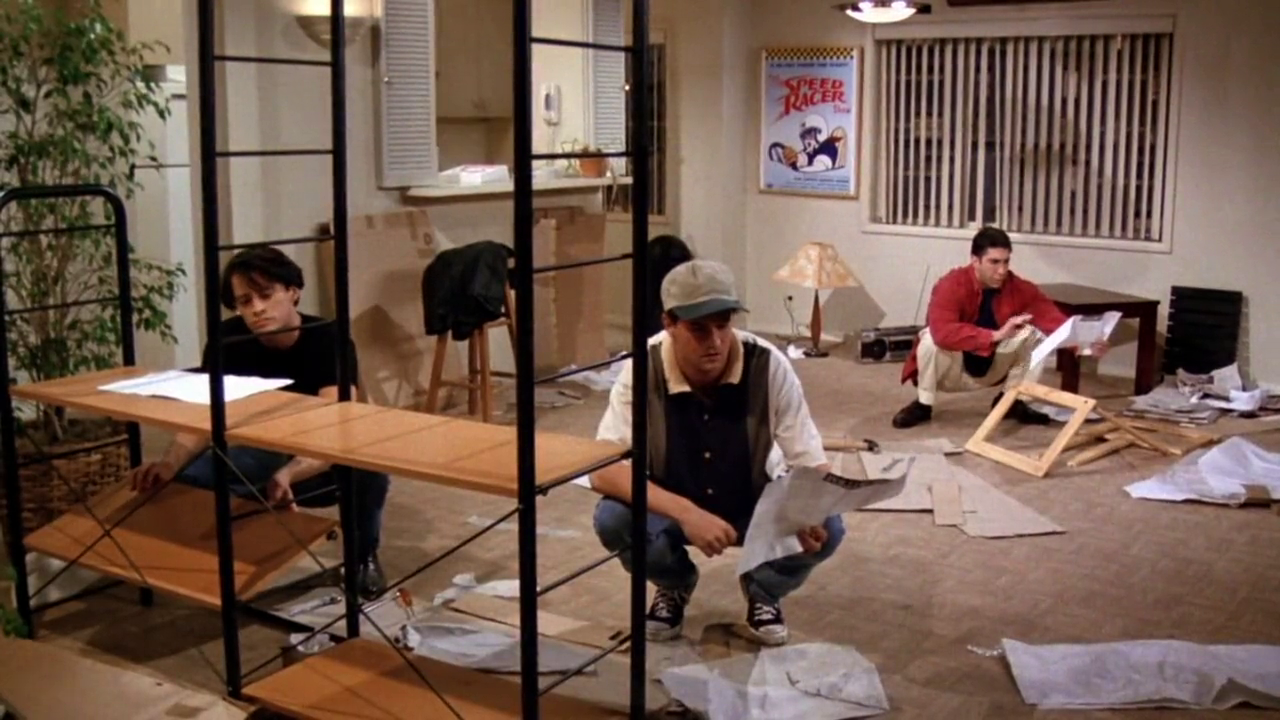
\includegraphics[trim={0 10cm 0 1cm,}, clip, width=\paperwidth]{./S01/img/1/speed-racer.png}
    \caption{Speed Racer\label{fig:speed-racer}}
  \end{adjustwidth}
\end{figure}

\saveparinfos
\noindent
\begin{minipage}[c]{0.5\textwidth}\useparinfo

No novo apartamento do Ross, é possível ver um poster de \emph{The Speed
Racer Show} (1967--1968) produzida pela \emph{Tatsunoko Production}.
Trata-se de uma série japonesa animada protagonizada por \emph{Go
Mifune}, conhecido como \emph{Speed Racer}. É baseada no mangá
\emph{Mach Go Go Go} (1966) criada por \emph{Tatsuo Yoshida}.

\end{minipage}\hfill
\begin{minipage}[c]{0.5\textwidth}

\begin{figure}
  \centering
  \begin{tikzpicture}
    \node [inner sep=0pt] at (0,0) {
      
\includegraphics[width=0.8\textwidth,keepaspectratio]{./S01/img/1/speed-racer-poster.jpeg}
    };
    \draw [white, rounded corners=\ClipSep, line width=\ClipSep]
    (current bounding box.north west) --
    (current bounding box.north east) --
    (current bounding box.south east) --
    (current bounding box.south west) -- cycle
    ;
    \end{tikzpicture}
    \caption{Speed Racer poster\label{fig:speed-racer-poster}}
\end{figure}

\end{minipage}

\hypertarget{referuxeancias-4}{%
\subsection{Referências}\label{referuxeancias-4}}

\begin{itemize}
\tightlist
\item
  \sloppy IMDB. \url{https://www.imdb.com/title/tt0061300/}
\item
  \sloppy Review do Omelete. \url{https://www.omelete.com.br/series-tv/lembra-desse-speed-racer-a-serie-original}
\item
  \sloppy Abertura (YouTube). \url{https://www.youtube.com/watch?v=suCm1w_KTiY}
\end{itemize}

\hypertarget{joanie-loves-chachi}{%
\section{Joanie Loves Chachi}\label{joanie-loves-chachi}}

\begin{figure}[!ht]
  \begin{adjustwidth}{-\oddsidemargin-1in}{-\rightmargin}
    \centering
    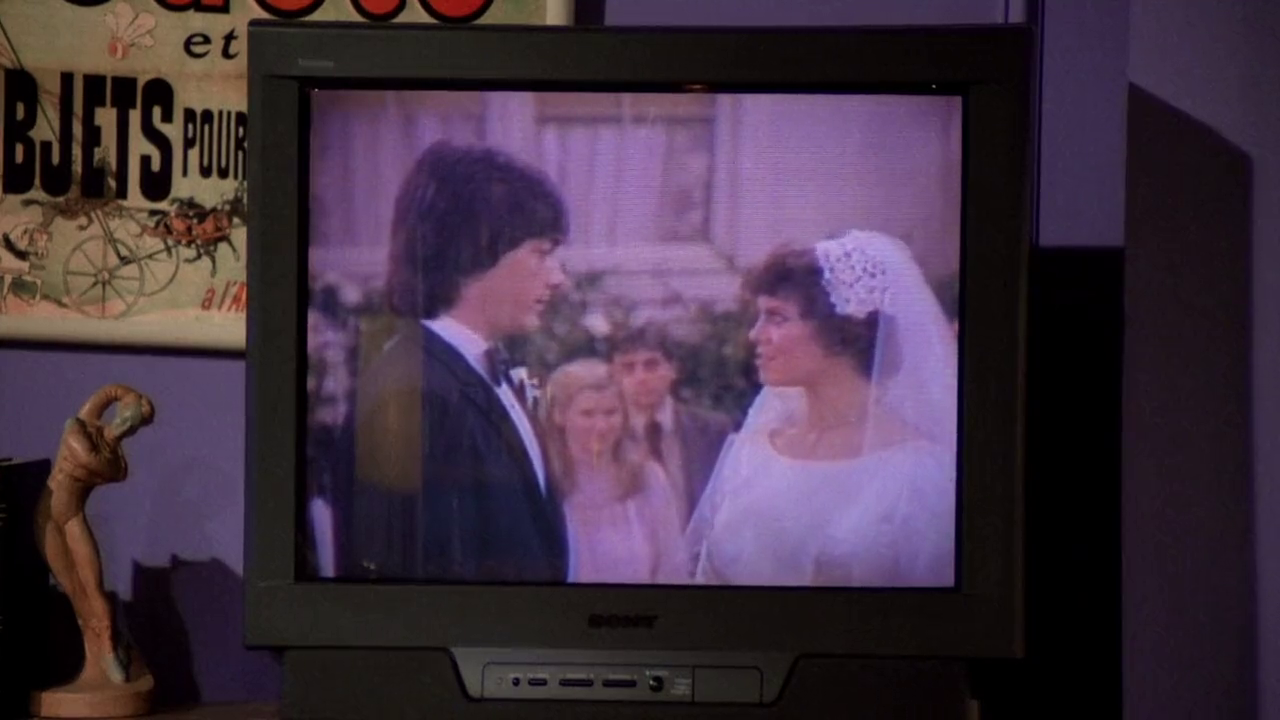
\includegraphics[trim={0 4cm 0 2cm,}, clip, width=\paperwidth]{./S01/img/1/joanie-loves-chachi.png}
    \caption{Joanie Loves Chachi\label{fig:joanie-loves-chachi}}
  \end{adjustwidth}
\end{figure}

\begin{tcolorbox}[enhanced,center upper,
    drop fuzzy shadow southeast, boxrule=0.3pt,
    lower separated=false,
    colframe=black!30!dialogoBorder,colback=white]
\begin{minipage}[c]{0.14\linewidth}
  \raisebox{\dimexpr-\height+\ht\strutbox\relax}{
    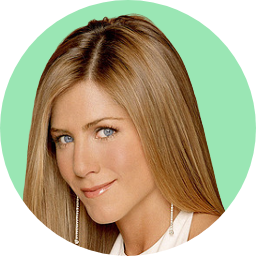
\includegraphics[width=1.5cm]{./assets/img/rachel.png}
  }
   & \centering \scriptsize{Rachel}
\end{minipage}
\hspace{.1mm}
\begin{minipage}[c]{0.8\linewidth}
  \textbf{- But Joanie loved Chachi. That's the difference.}\\
  - Mas Joanie ama Chachi. Essa é a diferença.
\end{minipage}
\end{tcolorbox}

No apartamento de Monica, Rachel, ainda em seu vestido de noiva, assiste
a \emph{Joanie Loves Chachi} (1982--1983) - \emph{spin off} de
\emph{Happy Days} (1974) -, uma série de TV que mostra as aventuras
românticas de Joanie Cunningham e Chachi Arcola, buscando uma carreira
musical em Chicago.

\hypertarget{referuxeancias-5}{%
\subsection{Referências}\label{referuxeancias-5}}

\begin{itemize}
\tightlist
\item
  \sloppy IMDB. \url{https://www.imdb.com/title/tt0083433/}
\item
  \sloppy Wikipédia. \url{https://en.wikipedia.org/wiki/Joanie_Loves_Chachi}
\end{itemize}

\hypertarget{billy-dont-be-a-hero}{%
\section{Billy, don't be a hero}\label{billy-dont-be-a-hero}}

\begin{figure}[!ht]
  \begin{adjustwidth}{-\oddsidemargin-1in}{-\rightmargin}
    \centering
    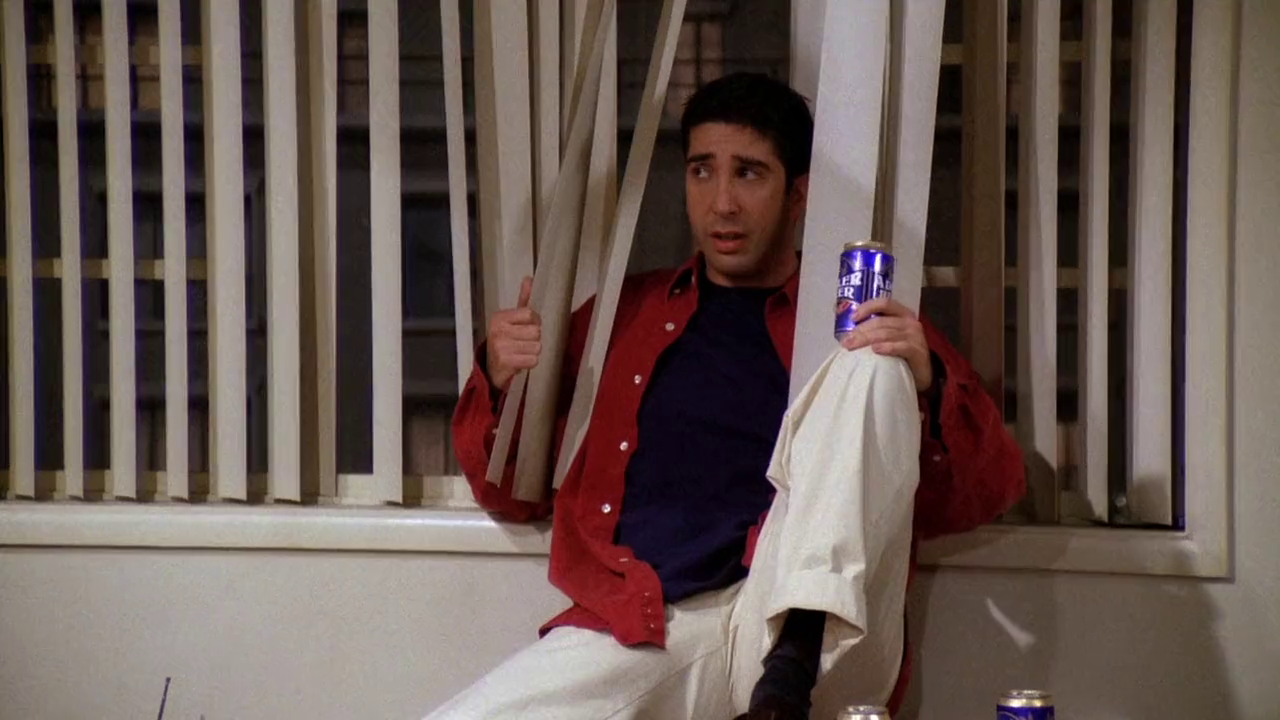
\includegraphics[trim={0 6.5cm 0 2.5cm,}, clip, width=\paperwidth]{./S01/img/1/billy-dont-be-a-hero.png}
    \caption{Billy, don’t be a hero\label{fig:billy-don-t-be-a-hero}}
  \end{adjustwidth}
\end{figure}

\begin{tcolorbox}[enhanced,center upper,
    drop fuzzy shadow southeast, boxrule=0.3pt,
    lower separated=false,
    colframe=black!30!dialogoBorder,colback=white]
\begin{minipage}[c]{0.14\linewidth}
  \raisebox{\dimexpr-\height+\ht\strutbox\relax}{
    
\includegraphics[width=1.5cm]{./assets/img/ross.png}
  }
   & \centering \scriptsize{Ross}
\end{minipage}
\hspace{.1mm}
\begin{minipage}[c]{0.8\linewidth}
  \textbf{- Do the words, 'Billy, don't be a hero', mean anything to you?}\\
  - As palavras, 'Billy, don't be a hero', significam alguma coisa pra vocês?
\end{minipage}
\end{tcolorbox}

\saveparinfos
\noindent
\begin{minipage}[c]{0.5\textwidth}\useparinfo

Ross faz menção a música \emph{Billy, don't be a hero} (1974) composta
por Mitch Murray e Peter Callander. Lançada inicialmente no Reino Unido
na voz de \emph{Paper Lace}, foi logo em seguida lançada também nos
Estados Unidos pelo grupo \emph{Bo Donaldson and The Heywoods.}

\end{minipage}\hfill
\begin{minipage}[c]{0.5\textwidth}

\begin{figure}
  \centering
  \begin{tikzpicture}
    \node [inner sep=0pt] at (0,0) {
      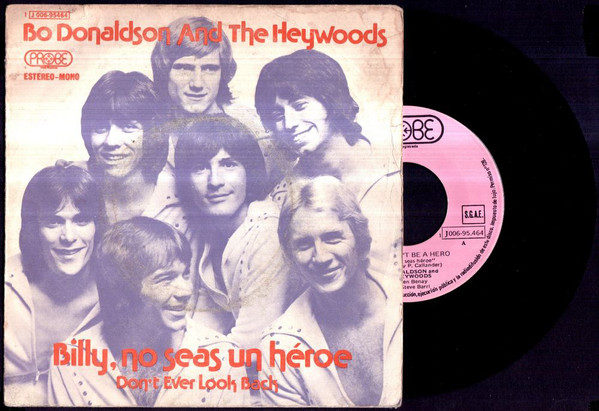
\includegraphics[width=0.8\textwidth,keepaspectratio]{./S01/img/1/billy-dont-be-a-hero-single.jpg}
    };
    \draw [white, rounded corners=\ClipSep, line width=\ClipSep]
    (current bounding box.north west) --
    (current bounding box.north east) --
    (current bounding box.south east) --
    (current bounding box.south west) -- cycle
    ;
    \end{tikzpicture}
    \caption{Billy, don’t be a hero - Single\label{fig:billy-don-t-be-a-hero-single}}
\end{figure}

\end{minipage}

\hypertarget{referuxeancias-6}{%
\subsection{Referências}\label{referuxeancias-6}}

\begin{itemize}
\tightlist
\item
  \sloppy Site Oficial. \url{http://www.bodonaldson.net/}
\item
  \sloppy IMDB. \url{https://en.wikipedia.org/wiki/Billy_Don%27t_Be_a_Hero}
\item
  \sloppy Letra - MetroLyrics. \url{https://www.metrolyrics.com/billy-dont-be-a-hero-lyrics-paper-lace.html}
\item
  \sloppy Billy, don’t be a hero - YouTube. \url{https://www.youtube.com/watch?v=1qlK9TJvuSk}
\end{itemize}

\hypertarget{pinocchio}{%
\section{Pinocchio}\label{pinocchio}}

\begin{figure}[!ht]
  \begin{adjustwidth}{-\oddsidemargin-1in}{-\rightmargin}
    \centering
    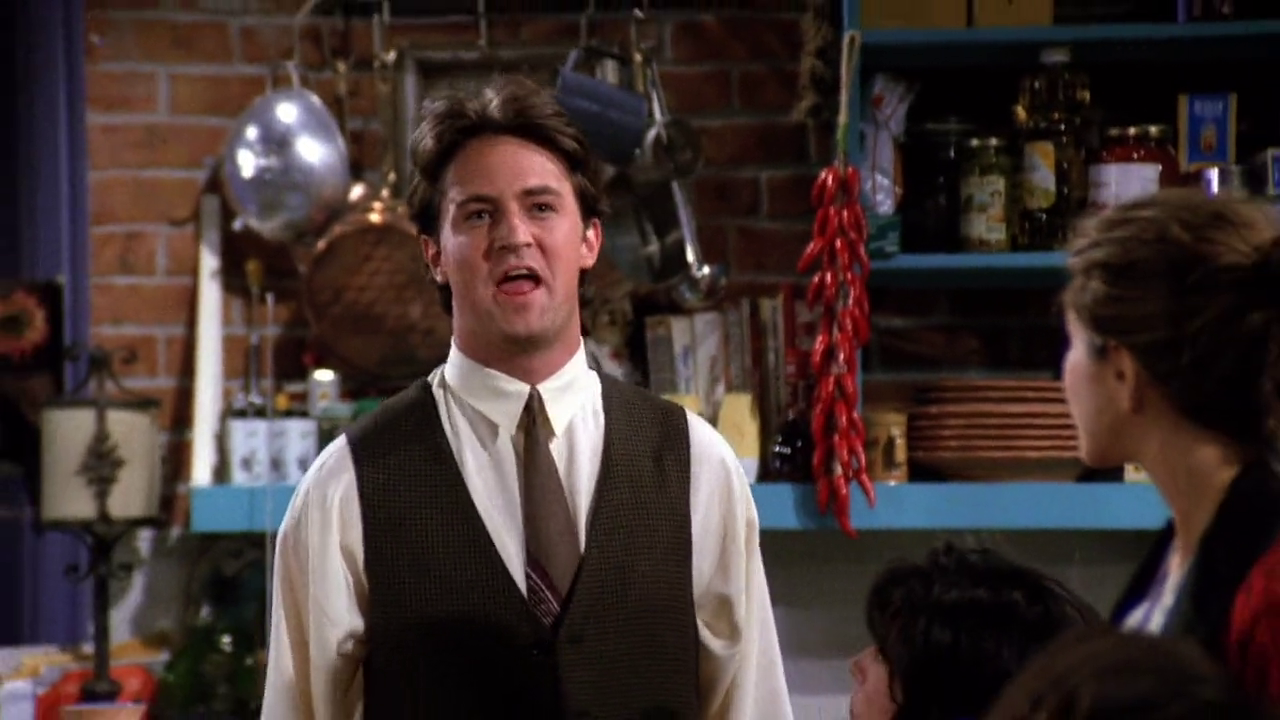
\includegraphics[trim={0 5cm 0 2cm,}, clip, width=\paperwidth]{./S01/img/1/pinocchio.png}
    \caption{Pinocchio\label{fig:pinocchio}}
  \end{adjustwidth}
\end{figure}

\begin{tcolorbox}[enhanced,center upper,
    drop fuzzy shadow southeast, boxrule=0.3pt,
    lower separated=false,
    colframe=black!30!dialogoBorder,colback=white]
\begin{minipage}[c]{0.14\linewidth}
  \raisebox{\dimexpr-\height+\ht\strutbox\relax}{
    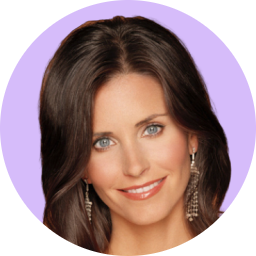
\includegraphics[width=1.5cm]{./assets/img/monica.png}
  }
   & \centering \scriptsize{Monica}
\end{minipage}
\hspace{.1mm}
\begin{minipage}[c]{0.8\linewidth}
  \textbf{- Wait, unless you happened to catch the Reruns' production of Pinocchio.}\\
  - Espera, a não ser que tenha visto a refilmagem do Pinóquio.
\end{minipage}

\medskip
\begin{minipage}[c]{0.14\linewidth}
  \raisebox{\dimexpr-\height+\ht\strutbox\relax}{
    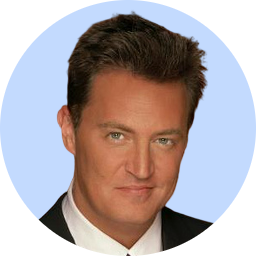
\includegraphics[width=1.5cm]{./assets/img/chandler.png}
  }
   & \centering \scriptsize{Chandler}
\end{minipage}
\hspace{.1mm}
\begin{minipage}[c]{0.8\linewidth}
  \textbf{- Look, Gepetto, I'm a real live boy.}\\
  - Olha, Gepetto, sou um menino de verdade.
\end{minipage}
\end{tcolorbox}

\saveparinfos
\noindent
\begin{minipage}[c]{0.5\textwidth}\useparinfo

Referência ao filme \emph{Pinocchio} (1940) ou \emph{Pinóquio} como
ficou conhecido no Brasil. Produzido pela \emph{Walt Disney}, o filme
conta a história de um velho carpinteiro chamado \emph{Gepetto}, que faz
um boneco de madeira chamado \emph{Pinóquio}, o qual é trazido a vida
pela \emph{Fada Azul}, com a condição de que ele demonstre obediência,
bravura e lealdade a seu criador.

\end{minipage}\hfill
\begin{minipage}[c]{0.5\textwidth}

\begin{figure}
  \centering
  \begin{tikzpicture}
    \node [inner sep=0pt] at (0,0) {
      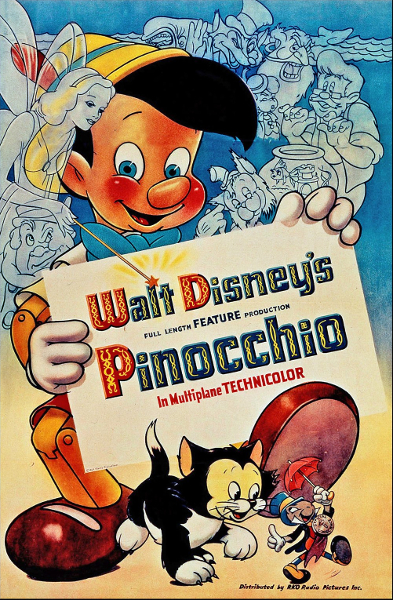
\includegraphics[width=0.5\textwidth,keepaspectratio]{./S01/img/1/pinocchio-poster.jpg}
    };
    \draw [white, rounded corners=\ClipSep, line width=\ClipSep]
    (current bounding box.north west) --
    (current bounding box.north east) --
    (current bounding box.south east) --
    (current bounding box.south west) -- cycle
    ;
    \end{tikzpicture}
    \caption{Pinocchio - Poster\label{fig:pinocchio-poster}}
\end{figure}

\end{minipage}

O filme tem muitos trechos musicais, e é daí que o Chandler retira
inspiração para a música que ele canta ao sair do apartamento:

\bigskip
\begin{tcolorbox}[enhanced,
    drop fuzzy shadow southeast, boxrule=0.3pt,
    lower separated=false, sidebyside, sidebyside align=top,
    halign=flush right, halign lower=left,
    colframe=black!30!dialogoBorder,colback=musicaBg]
\includegraphics[width=0.4cm]{./assets/img/icon-music.png}\\
Once I was a wooden boy,\\a little wooden boy…\\
\tcblower
\includegraphics[width=0.4cm]{./assets/img/icon-language.png}\\
Uma vez eu era um garoto de madeira,\\Um pequeno garoto de madeira…\\
\end{tcolorbox}

\hypertarget{referuxeancias-7}{%
\subsection{Referências}\label{referuxeancias-7}}

\begin{itemize}
\tightlist
\item
  \sloppy IMDB. \url{https://www.imdb.com/title/tt0032910/}
\item
  \sloppy Wikipédia. \url{https://pt.wikipedia.org/wiki/Pin%C3%B3quio_(filme)}
\end{itemize}

\hypertarget{liza-minnelli}{%
\section{Liza Minnelli}\label{liza-minnelli}}

\begin{figure}[!ht]
  \begin{adjustwidth}{-\oddsidemargin-1in}{-\rightmargin}
    \centering
    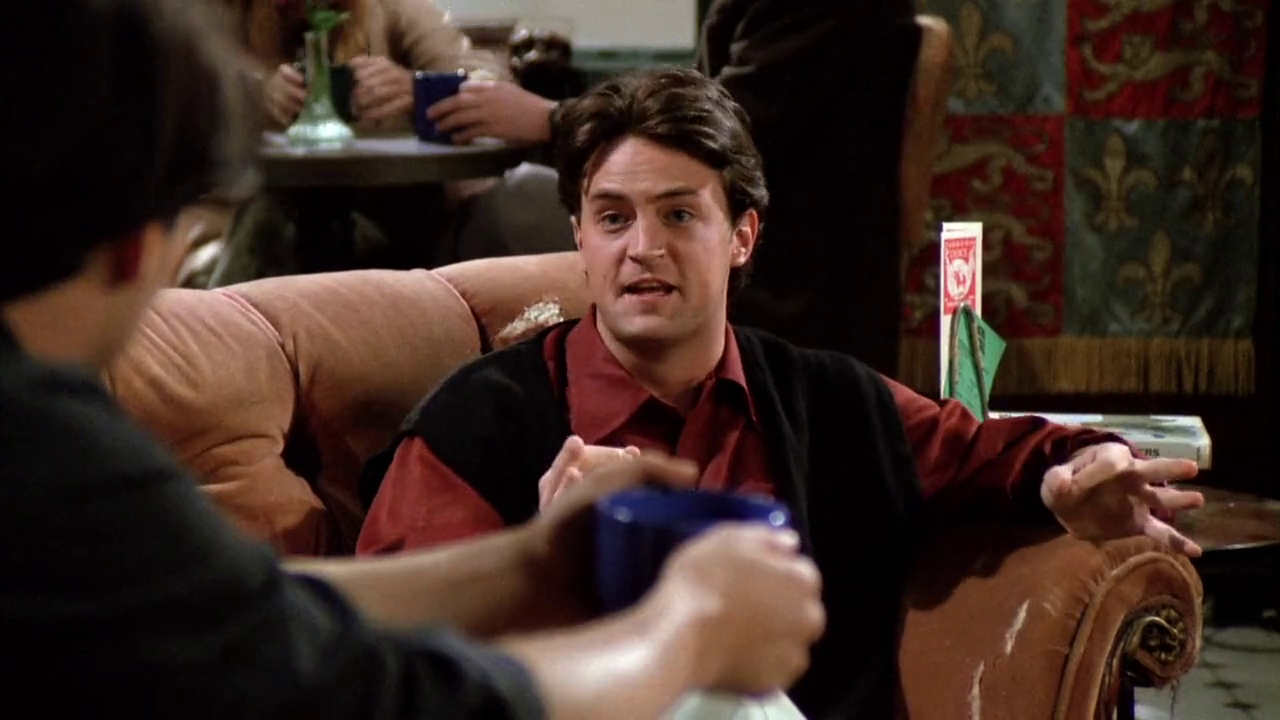
\includegraphics[trim={0 5cm 0 2cm,}, clip, width=\paperwidth]{./S01/img/1/liza-minnelli.png}
    \caption{Liza Minnelli\label{fig:liza-minnelli}}
  \end{adjustwidth}
\end{figure}

\begin{tcolorbox}[enhanced,center upper,
    drop fuzzy shadow southeast, boxrule=0.3pt,
    lower separated=false,
    colframe=black!30!dialogoBorder,colback=white]
\begin{minipage}[c]{0.14\linewidth}
  \raisebox{\dimexpr-\height+\ht\strutbox\relax}{
    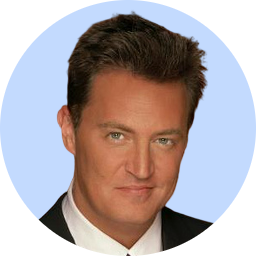
\includegraphics[width=1.5cm]{./assets/img/chandler.png}
  }
   & \centering \scriptsize{Chandler}
\end{minipage}
\hspace{.1mm}
\begin{minipage}[c]{0.8\linewidth}
  \textbf{- Kids, new dream. I'm in Las Vegas. I'm Liza Minnelli.}\\
  - Crianças, novo sonho. Tô em Las Vegas. Eu sou Liza Minelli.
\end{minipage}
\end{tcolorbox}

\saveparinfos
\noindent
\begin{minipage}[c]{0.5\textwidth}\useparinfo

Chandler menciona a atriz e cantora americana \emph{Liza Minnelli}
(1946-), é conhecida por ganhar o Oscar de melhor atriz por sua atuação
no filme \emph{Cabaret} (1972).

\end{minipage}\hfill
\begin{minipage}[c]{0.5\textwidth}

\begin{figure}
  \centering
  \begin{tikzpicture}
    \node [inner sep=0pt] at (0,0) {
      
\includegraphics[width=0.8\textwidth,keepaspectratio]{./S01/img/1/liza-minnelli-cabaret.jpg}
    };
    \draw [white, rounded corners=\ClipSep, line width=\ClipSep]
    (current bounding box.north west) --
    (current bounding box.north east) --
    (current bounding box.south east) --
    (current bounding box.south west) -- cycle
    ;
    \end{tikzpicture}
    \caption{Liza Minnelli - Cabaret\label{fig:liza-minnelli-cabaret}}
\end{figure}

\end{minipage}

\hypertarget{referuxeancias-8}{%
\subsection{Referências}\label{referuxeancias-8}}

\begin{itemize}
\tightlist
\item
  \sloppy IDMB. \url{https://www.imdb.com/name/nm0591485/}
\item
  \sloppy Wikipédia. \url{https://pt.wikipedia.org/wiki/Liza_Minnelli}
\end{itemize}


%----------------------------------------------------------------------------------------
%	BIBLIOGRAPHY
%----------------------------------------------------------------------------------------

\chapter*{Bibliography}
\addcontentsline{toc}{chapter}{\textcolor{ocre}{Bibliography}} % Add a Bibliography heading to the table of contents

%------------------------------------------------

\section*{Articles}
\addcontentsline{toc}{section}{Articles}
\printbibliography[heading=bibempty,type=article]

%------------------------------------------------

\section*{Books}
\addcontentsline{toc}{section}{Books}
\printbibliography[heading=bibempty,type=book]

%----------------------------------------------------------------------------------------
%	INDEX
%----------------------------------------------------------------------------------------

\cleardoublepage % Make sure the index starts on an odd (right side) page
\phantomsection
\setlength{\columnsep}{0.75cm} % Space between the 2 columns of the index
\addcontentsline{toc}{chapter}{\textcolor{ocre}{Index}} % Add an Index heading to the table of contents
\printindex % Output the index

%----------------------------------------------------------------------------------------

\end{document}
